%%% Dichiarazione dei pacchetti standard.
\documentclass{beamer}
\usepackage[utf8]{inputenc}
\usepackage[italian]{babel}
\usepackage{graphicx}

\usepackage{amsfonts}
%\usepackage[square, numbers, comma, sort&compress]{natbib}  % Use the
                                % "Natbib" style for the references in
                                % the Bibliography

%%% Personalizzazione del layout---articolata su cinque livelli.
%\usetheme{split}        % layout complessivo. 
%\usetheme{Goettingen}        % layout complessivo. 
%\usetheme{CambridgeUS}        % layout complessivo. 
%\usetheme{Boadilla}        % layout complessivo. 
%\usetheme{Montpellier}        % layout complessivo. 
%\usetheme{Warsaw}        % layout complessivo. 
%\usetheme{Pittsburgh}        % layout complessivo. 
\usetheme{Hannover}        % layout complessivo. 

\useinnertheme{default} % layout interno.
\useoutertheme{default} % layout esterno.
\usecolortheme{default} % schema di colori.
\usefonttheme{default}  % schema dei font.
% Inutile dire che se volete tutti i default, potete risparmiarvi gli ultimi
% quattro comandi. 


%%% Titolo e autore.

\title{Reti federate eventualmente connesse}
\subtitle{Architettura e prototipo per la Rete Mocambos}
\author{Vincenzo Tozzi}
\institute{Universit\`a degli Studi di Firenze - Corso di Laurea in Informatica}
\date{23 aprile 2012}

\begin{document}

% Local background must be enclosed by curly braces for grouping.
{
\usebackgroundtemplate{
  \hspace{0.02cm}
  
\includegraphics[width=.3\textwidth]{./Figure/logoUNIFI.pdf}
}%
\begin{frame}
  \titlepage
\end{frame}
}

\section[Sommario]{}
\begin{frame}
  \tableofcontents
\end{frame}

\section{Introduzione}
\begin{frame}

  \frametitle{Brasile: Uno, nessuno e centomila}
  Il Brasile è un paese di dimensione continentale dove convivono
  molte culture in ambienti e contesti molto diversi. 
  \begin{itemize}
  \item Indios
  \item Quilombola
  \item Caiçaras
  \item Riberinhos
  \item \ldots
  \end{itemize}

\end{frame}

\begin{frame}

  \frametitle{Digital divide - Inclusão digital}
  Popolazione con accesso ad Internet in Brasile\footnote{Fonte: intervista al Segretario Esecutivo del Ministero delle
    Comunicazioni, Cesar Alvarez, su dati IBGE 2009.}:
  \begin{itemize}
    \item $\sim$ 30\% della popolazione
    \item $\sim$ 6\% della popolazione in area rurale  
  \end{itemize}
    
\end{frame}

\begin{frame}

  \frametitle{Come si affronta il digital divide?}
  \begin{itemize}
    \item Alfabetizzazione informatica
    \item Accesso a internet
    \item e poi\ldots
    \item Ricerca e sviluppo?
    \end{itemize}

 \end{frame}

\begin{frame}

  \frametitle{Neutralità tecnologica}

  \begin{quote}
    ``Siamo portati a pensare al mezzo come neutrale, ma se prendiamo
    ad esempio i principali e più diffusi mezzi di comunicazione, le
    lingue, possiamo intuire come queste non siano interscambiabili
    essendo l'espressione delle culture e delle società che le usano e
    le vivono.''
  \end{quote}
  
\end{frame}


\begin{frame}
  \frametitle{Internet, autonomia e libertà tecnologica}
  \framesubtitle{Dagli RFC\ldots}
  \begin{quote}
  ``Internet è nata dal confronto aperto tra i responsabili di diverse
  reti, uniti dalla volontà di connettere le loro differenti
  realtà. La nascita di nuovi servizi, per queste reti eterogenee, era
  basata sulla discussione e il confronto. Il primo uso documentato
  del termine ``internet'', seguendo questa pratica, fa la sua
  comparsa proprio in un RFC'' 
\end{quote}

\end{frame}

\begin{frame}
  \frametitle{Internet, autonomia e libertà tecnologica}
  \framesubtitle{\ldots ai ToS/API/Cloud}
  \begin{quote}
  ``Negli ultimi anni la diffusione della banda larga, ma sopratutto
  strategie come quella adottata da Google, hanno  trasformato il 
  concetto stesso di internet che da rete globale di reti eterogenee,
  diventa principalmente una rete per la globalizzazione di servizi
  fortemente centralizzati e uniformati.'' 
  \end{quote}
\end{frame}


\section{Reti federate eventualmente connesse}

\begin{frame}
  \frametitle{La Rete Mocambos}
  \begin{itemize}
    \item Più di 200 comunità rurali sparse su tutto il territorio
      nazionale, principalmente in zone amene
    \item Comunità di matrice africana (quilombos) e indigena (aldeias)
    \item Uso critico e autonomo di TIC
    \item Banda disponibile limitata (connessioni satellitari 512/128 Kbps)
    \end{itemize}
\end{frame}


\begin{frame}
  \frametitle{Reti federate eventualmente connesse}
  \begin{quotation}
    ``una rete federata basata su connessioni non sempre disponibili,
    quali le connessioni satellitari, con l'esigenza di mantenere i
    servizi federati attivi, anche in assenza di comunicazione. I
    servizi federati sono inoltre ottimizzati per la resilienza del
    sistema e la riduzione del traffico di rete esterno, attraverso
    strategie di replicazione, sincronizzazione e memorizzazione dei
    dati sull'infrastruttura logica/fisica locale.''
    \end{quotation}
\end{frame}


% Local background must be enclosed by curly braces for grouping.
{
%\usebackgroundtemplate{\includegraphics[width=.4\textwidth]{include/pista.jpg}}%
\begin{frame}
  \frametitle{Reti federate eventualmente connesse}
  \framesubtitle{Tecnologie e strumenti utili}
  \begin{itemize}
    \item LDAP
    \item XMPP
    \item OpenID
    \item OAuth
    \item Django / Ruby On Rails
    \item git / git-annex
    \item rsync
    \end{itemize}

\end{frame}
}


\section{Un'architettura per la Rete Mocambos}

\begin{frame}
  \frametitle{Un'architettura per la Rete Mocambos}
  \framesubtitle{Specifica dei requisiti}
  \begin{itemize}
    \item Identità di rete
    \item Autenticazione decentrata
    \item Sincronizzazione
    \item Riproducibilità
    \item Manutenzione
    \item Sviluppo
    \end{itemize}

\end{frame}

\begin{frame}
  \frametitle{Un'architettura per la Rete Mocambos}
  \framesubtitle{Strumenti e pratiche per lo sviluppo}
  \begin{itemize}
    \item Documentazione e ``versionamento'': wiki, git
    \item Sistema operativo: Debian e Ubuntu
    \item Linguaggi di programmazione: Python, shell script
    \item Virtualizzazione: Virtualbox, Virtualenv
    \end{itemize}

\end{frame}

\begin{frame}
  \frametitle{Un'architettura per la Rete Mocambos}
  \framesubtitle{Architettura di base}
	\begin{figure}
		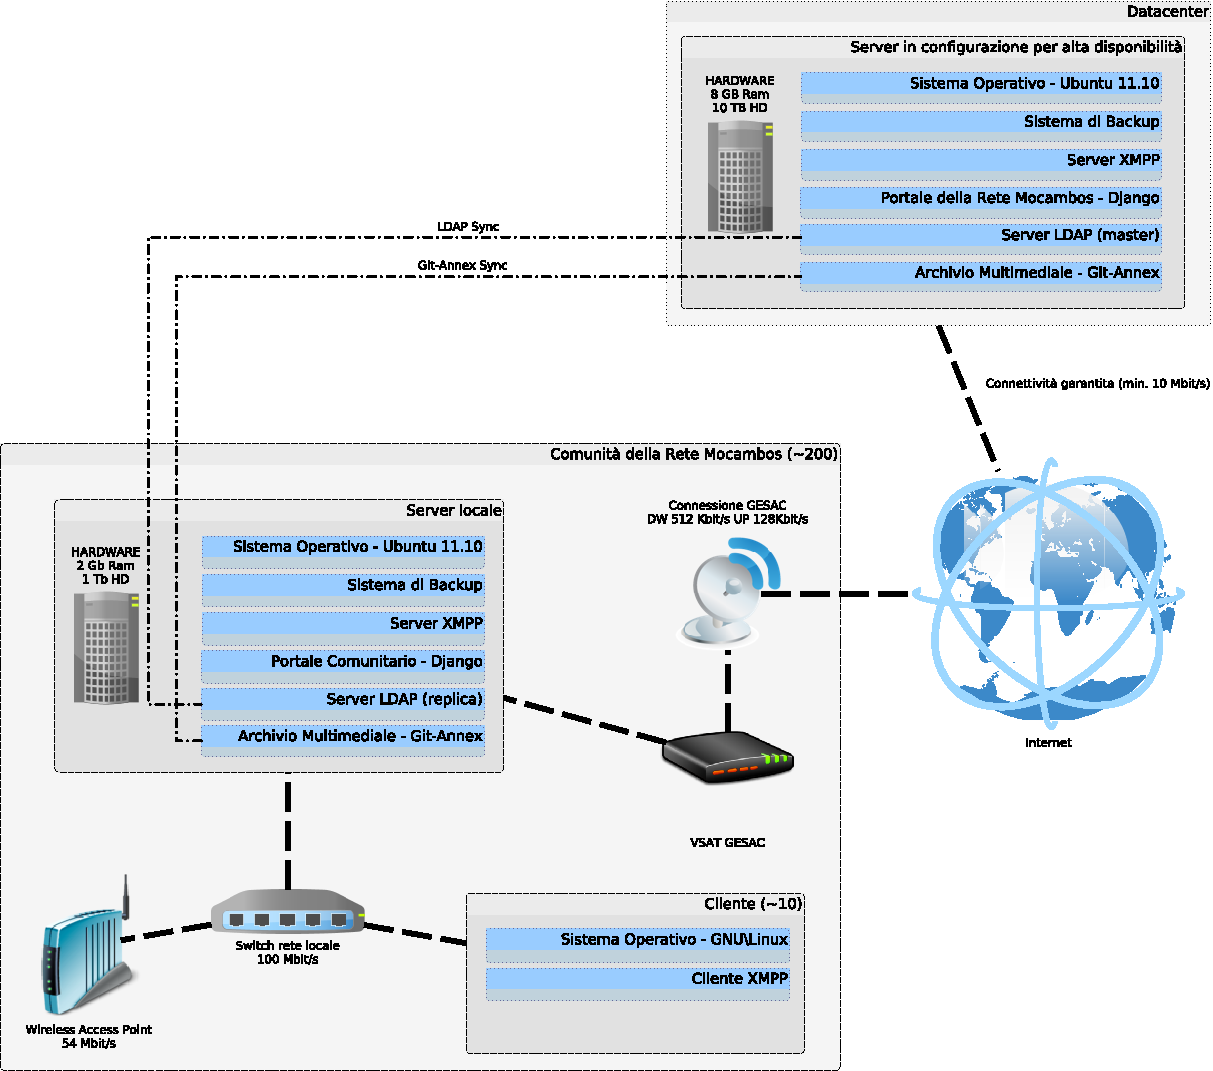
\includegraphics[height=0.7\textheight]{./Figure/SchemaServer_ReteMocambos-crop.pdf}
	\end{figure}


\end{frame}

\section{Un prototipo di servizio federato}

\begin{frame}
  \frametitle{Un prototipo di servizio federato}
  \framesubtitle{Sistema di pubblicazione e diffusione di contenuti multimediali}

\end{frame}

\begin{frame}
  \frametitle{Un prototipo di servizio federato}
  \framesubtitle{Archivio multimediale}

\end{frame}

\section{Conclusioni e sviluppi futuri}

\begin{frame}[fragile]
 \frametitle{Conclusioni e sviluppi futuri}
%  \framesubtitle{}

\end{frame}


\end{document}

%	\begin{figure}
%		\includegraphics[width=\textwidth]{include/albero_tempi.pdf}
%	\end{figure}
